\question (北京邮电大学,2005年)理想情况下,散列表的平均比较次数为( )
\par\twoch{\textcolor{red}{1}}{2}{4}{n}
\begin{solution}散列表是根据给定的关键字来计算出关键字在表中的地址,因此理想情况下,散列表的平均比较次数为1次。
\end{solution}
\question (南开大学,2005年)假定关键字K=2789465,允许存储地址为3位十进制数,现在得到的散列地址为149,则所采用的构建散列函数的方法是(
)
\par\twoch{除留余数法,模为23}{\textcolor{red}{平方取中法}}{移位叠加法}{间界叠加法}
\begin{solution}2789465的平方为7781114986225,其中间3位为149,所以采用的是平方取中法。
本题还可使用排除法,A较好排除,C、D均不是常用的散列函数构造方法,所以选择B。
\end{solution}
\question (中国科学院自动化所)设散列地址空间为0~m-1,k为关键字,用p去除k,将所得到的余数作为k的散列地址,即H(k)=k
mod p,为了减少发生冲突的概率,一般取p为( )
\par\twoch{小于m}{小于m的最大偶数}{m}{\textcolor{red}{小于m的最大素数}}
\begin{solution}p取小于m的最大素数,这样可以使得冲突的概率降到最小。
\end{solution}
\question 为提高散列(Hash)表的查找效率,可以采取的正确措施是( )。
\ding{192}.增大装填(载)因子 \ding{193}.设计冲突(碰撞)少的散列函数
\ding{194}.处理冲突(碰撞)时避免产生聚集(堆积)现象
\par\twoch{仅\ding{192}}{仅\ding{193}}{仅\ding{192}、\ding{193}}{\textcolor{red}{仅\ding{193}、\ding{194}}}
\begin{solution}装填(载)因子越大,发生冲突的可能性越大,所以\ding{192}错误。因为散列表是由散列函数和处理冲突两部分组成的,查找效率与这两部分有关,所以\ding{193}和\ding{194}是正确的。
【总结】
查找过程中,关键码的比较次数取决于产生冲突的多少,产生的冲突少,查找效率就高;产生的冲突多,查找效率就低。因此,影响产生冲突多少的因素,也就是影响查找效率的因素。影响产生冲突多少的因素有以下3个:
1)散列函数是否均匀。 2)处理冲突的方法。 3)散列表的装填因子。
\end{solution}
\question 用哈希(散列)方法处理冲突(碰撞)时可能出现堆积(聚集)现象,下列选项中,会受堆积现象直接影响的是(
)
\par\twoch{存储效率}{散列函数}{装填(装载)因子}{\textcolor{red}{平均查找长度}}
\begin{solution}聚集现象即产生了冲突,每次冲突就会增加查找的次数,因此会增加平均查找长度。
\end{solution}
\question (华中科技大学,2006年)一组关键字(87,73,25,55,90,28,31,17,101,22,3,62),若哈希函数为H(key)=key
MOD 11,在链地址法处理后的同一链表中的是( )
\par\twoch{81,90}{31,101}{3,78}{\textcolor{red}{62,73}}
\begin{solution}在链地址法处理后同处于同一链表中只需MOD 11的余数相同
\end{solution}
\question (青岛大学,2004年)设哈希表长m=18,哈希函数H(K)=K\%17。关键字序列为:\{53,17,12,61,98,70,87,25,63,46,14,59,67,75\},如果使用二次探测再散列处理冲突,则查找成功的平均查找长度约为(
)
\par\twoch{\textcolor{red}{2.18}}{1.71}{2.96}{1.06}
\begin{solution}根据散列函数以及处理冲突的方法,计算查找每个节点的成功时的查找次数,在计算平均值,得所求结果为2.18
\end{solution}
\question (中科院,2006年)采用开放定址法解决冲突的哈希表中,发生聚集的原因主要是(
)
\par\twoch{数据元素过多}{负载因子过大}{哈希函数选择不当}{\textcolor{red}{解决冲突的算法不好}}
\begin{solution}散列地址不同的节点争夺同一个后继散列地址的现象称为聚集或堆积。这将造成不适同义词的节点也处在同一个探查序列之中,从而增加了探查序列的长度,即增加了查找时间。主要原因是算法选择的问题,如果用二次探测再散列法,则聚集的程度会远小于线性探测再散列法
\end{solution}
\question (华南理工大学,2005年)在构造哈希表方面,下面的说法( )是正确的
\par\fourch{链地址法在处理冲突时会产生聚集}{\textcolor{red}{线性探测再散列在处理冲突时会产生聚集}}{好的哈希函数可以完全避免冲突}{在哈希表中进行查找是不需要关键字比较的}
\begin{solution}A.链地址法就是为了处理聚集而动态的生成链表记录地址。B线性探测再散列会产生聚集,冲突发生时,顺序查看表中下一单元,直到找出一个空单元或查遍全表。C哈希函数一般是由大的空间映射到小空间,所以冲突难以避免。D哈希表查找过程中需要进行关键字的比较以确定查找是否成功。
\end{solution}
\question (中南大学,2004年)Hash函数应当以( )取其值域的每个值
\par\twoch{最大概率}{最小概率}{平均概率}{\textcolor{red}{等概率}}
\begin{solution}设置Hash函数的目的就是将关键字能够均匀地散列到哈希表中,所以应当等概率地取其值域的每个值
\end{solution}
\question (中科院自动化所)设哈希地址空间为0\textasciitilde{}m-1,k为关键字,用p去除k,将所得的余数作为k的散列地址,即H(k)=k
mod p。为了减少发生冲突的概率,一般取p为( )
\par\twoch{小于m}{小于m的最大偶数}{m}{\textcolor{red}{小于m的最大素数}}
\begin{solution}p一般取小于m的最大素数,这样可以使得冲突的概率降到最小
\end{solution}
\question (武汉大学,2005年)在散列文件的建立与检索过程中,哈希地址是一个( )
\par\twoch{逻辑记录号}{基桶号}{数据区首址}{\textcolor{red}{索引区首址}}
\begin{solution}哈希地址是一个索引区的首地址
\end{solution}
\question (青岛大学,2005年)设哈希表长m=14,哈希函数H(k)=k\%11.表中已有4个关键字,如果使用二次探测再散列处理冲突,关键字为49的存储地址为(
~)
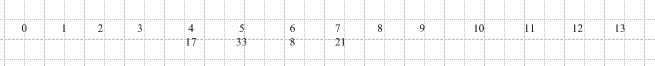
\includegraphics[width=3.33333in,height=0.33333in]{computerassets/3d96db8ff2bac40204c152331f211bb3.png}
\par\twoch{3}{5}{8}{\textcolor{red}{9}}
\begin{solution}取5时冲突,取5+1时又冲突,取5-1=4时也冲突,最后取5+4=9存储成功
\end{solution}
